\documentclass[border=2pt]{standalone}
\usepackage{circuitikz}
\begin{document}
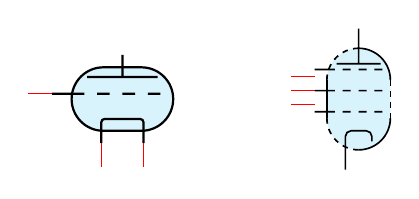
\begin{tikzpicture}
  \ctikzset{tubes/scale=.8,tubes/width=1.6,tubes/height=1,
    tubes/tube radius=.36,tubes/grid shift=.12,tubes/grid dashes=3,
    tubes/grid protrusion=.18,tubes/cathode width=.3,
    tubes/anode width=.5,tubes/anode distance=.5,
    tubes/cathode distance=.45,tubes/cathode corners=.08,
    tubes/cathode right extend=.15,tubes/fill=cyan!15}
  \node[triode,fullcathode] (T) at (0,0) {};
  \draw[red] (T.control) -- ++(-.3,0) (T.cathode 1) -- ++(0,-.3) (T.cathode 2) -- ++(0,-.3);
  \node[pentode,circuitikz/tubes/width=1,circuitikz/tubes/height=1.6,
    circuitikz/tubes/grid separation=.3,circuitikz/tubes/partial borders=121212,
    circuitikz/tubes/thickness=1.5] (P) at (3,0) {};
  \draw[red] (P.control) -- ++(-.3,0) (P.screen) -- ++(-.3,0) (P.suppressor) -- ++(-.3,0);
\end{tikzpicture}
\end{document}
